\documentclass[10pt,a4paper]{article}
\usepackage[latin1]{inputenc}
\usepackage{amsmath}
\usepackage{amsfonts}
\usepackage{amssymb}
\usepackage{graphicx}
\usepackage[obeyspaces]{url}
\usepackage[colorlinks,urlcolor=blue]{hyperref}

\title{Windows installation guide for fe-safe 2016}
\date{} % blank date

\begin{document}
	\maketitle
	
	\section*{Compatibility with Abaqus}
	fe-safe 2016 is compatible with Abaqus 2016. It will not work with Abaqus 6.14 and below.
	
	\section{Licence Requirements}
	Before installing fe-safe please read the \href{https://www.applications.itservices.manchester.ac.uk/show_product.php?id=338&tab=licensing}{licence requirements}, in particular noting:
	
	Only appropriately authorised support staff may make physical copies of the software or documentation.
	fe-safe may only be installed on computers owned by the University of Manchester; it may not be installed on computers owned by staff or students.
	With limited exceptions use of fe-safe by students is restricted to on-campus facilities.
	fe-safe on-line documentation may not be made available over the open internet.
	
	
	\section{Installation guide}
	\subsection{Documentation}
	Abaqus 2016 and fe-safe 2016 have the same documentation installer - see section 3.1 of the  \href{https://www.applications.itservices.manchester.ac.uk/medialibrary/docs/Abaqus/abaqus2016_windows_installation_guide.pdf}{Abaqus 2016 installation guide} for guidance. 
	
	
	\subsection{Software}
	\begin{itemize}
		\itemsep0em
		\item Mount the \path{fesafe_2016_Win_Lin.iso} file (e.g. using Virtual Clonedrive).
		\item Navigate to \path{\SIMULIA_fe-safe\1\windows} and run \textbf{setup.exe}.
		\item Accept the defaults until you reach the licensing section.
		\item \textbf{Licensing type} should be \textbf{Network} - this is the default selection.
		\item Under \textbf{Licensing system} select \textbf{FlexNet Licensing} from the dropdown menu - the default choice is \textbf{DSLS Licensing}.
		
		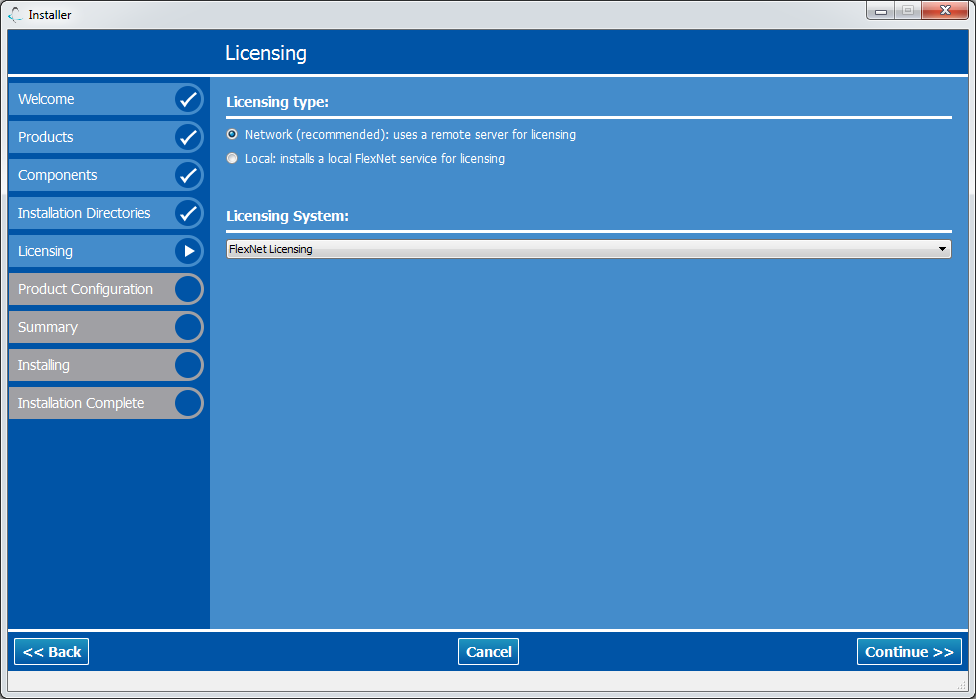
\includegraphics[width=0.9\textwidth]{fesafe_flexnet}
		
		\item Keep accepting the defaults by clicking \textbf{continue} until the installation is complete.
		\item Click on \textbf{finish}.
	\end{itemize}
			 
		
	The first time you start fe-safe you will be asked for network licence details. \textbf{Simulia FlexNet} is the type of licensing system to use, and you need to select \textbf{Network licence}, rather than \textbf{local licence}. Then in the box, type \path{lfarm4.its.manchester.ac.uk}, and in the drop down next to it, select all the text (which says \textbf{Default (27000)}, type \textbf{28003}), and leave the box checked next to \textbf{Save licence details}.
	
	\medskip
	
	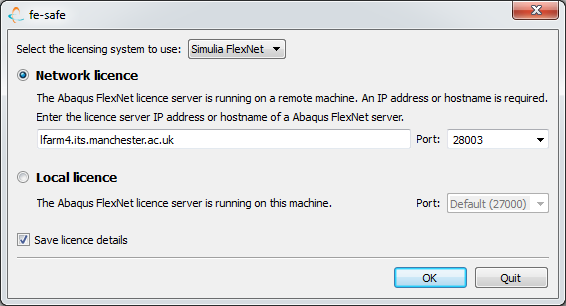
\includegraphics[width=0.9\textwidth]{fesafe_enter_licence_details}
\end{document}	